\documentclass[a4paper,12pt]{article}
\usepackage[english]{babel}
\usepackage[utf8]{inputenc}
\usepackage{setspace}

% Larger borders -- we do not want do waste paper, even if it is only paper on screen =)
\usepackage[top=2cm, bottom=2cm, left=2cm, right=2cm]{geometry}
% Remove auto indentation of paragraphs.
\setlength\parindent{0pt}

% Palatino font (nicer serif font: Times is for oldies)
%\renewcommand*\rmdefault{ppl}

% Nested itemize list bullet style
\renewcommand{\labelitemi}{$\bullet$}
\renewcommand{\labelitemii}{$\circ$}
\renewcommand{\labelitemiii}{--}

% Math packages
\usepackage{mathtools}
\usepackage{amsmath}
\usepackage{amsfonts}
\usepackage{amssymb}

% Graphic packages
\usepackage{graphicx}
\usepackage{subcaption}
\usepackage{float}
\usepackage{adjustbox}
\usepackage{tikz}
\usepackage{forest,array}
\usetikzlibrary{shadows}


% Graphs styles
\forestset{
  giombatree/.style={
    for tree={
      grow = east,
      parent anchor=east,
      child anchor=west,
      edge={rounded corners=2mm},
      fill=violet!5,
      drop shadow,
      l sep=10mm,
      edge path={
        \noexpand\path [draw, \forestoption{edge}] (!u.parent anchor) -- +(5mm,0) -- (.child anchor)\forestoption{edge label};
      }
    }
  }
}
\forestset{
  qtree/.style={
    for tree={
      parent anchor=south,
      child anchor=north,
      align=center,
      edge={rounded corners=2mm},
      fill=violet!5,
      drop shadow,
      l sep=10mm,
    }
  }
}

% BAN logic macros
\newcommand{\believes}{\mid\!\equiv}
\newcommand{\sees}{\triangleleft}
\newcommand{\oncesaid}{\mid\!\sim}
\newcommand{\controls}{\Rightarrow}
\newcommand{\fresh}[1]{\#(#1)}
\newcommand{\combine}[2]{{\langle #1 \rangle}_{#2}}
\newcommand{\encrypt}[2]{{ \{ #1 \} }_{#2}}
\newcommand{\sharekey}[1]{\xleftrightarrow{#1}}
\newcommand{\pubkey}[1]{\xmapsto{#1}}
\newcommand{\secret}[1]{\xleftrightharpoons{#1}}

\newcommand{\projectname}{Aeronautical Communication System}
\newcommand{\projectnameabbr}{ACS}

% Hides ugly links from the index
\usepackage[hidelinks]{hyperref}
% Landscape format pdf pagess
\usepackage{pdflscape}

\begin{document}
\pagenumbering{gobble}

{\setstretch{1.0}
  \begin{titlepage}
  	\centering
  	
\includegraphics[width=6cm]{img/unipi.pdf}\par
    \vspace{1.5cm}
    {\Large Department of Information Engineering \par}
  	\vspace{1.5cm}
  	{\huge\textsc{\projectname{}}\par}
    \vspace{0.5cm}
    {\Large Performance Evaluation of Computer Systems and Networks project \par}
  	\vspace{2cm}
  	Pietro \textsc{Gronchi}\par
  	Amedeo \textsc{Pochiero}\par
    Giovan Battista \textsc{Rolandi}

  	\vfill

    % Bottom of the page
  	{\large A.Y. 2019-2020\par}
  \end{titlepage}
}


\clearpage
\tableofcontents
\clearpage
\pagenumbering{arabic}

\section{Introduction} \label{Introduction}
\projectname{} is a communication system between aircrafts (AC) and a control tower (CT).
Connection between AC and CT is provided by ground base stations (BS), which are deployed over a grid, at a distance M from neighbors.

\begin{figure}[H]
  \centering
  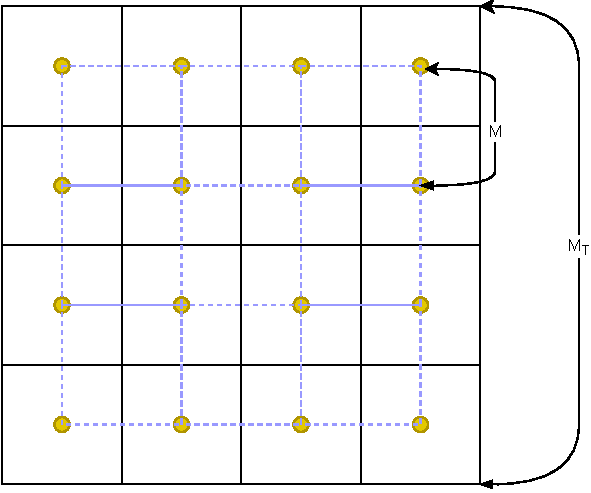
\includegraphics[scale=0.5]{img/grid.pdf}
  \caption{System topology}
  \label{fig:grid}
\end{figure}

Deployment grid has a square topology, eg. number of rows is equal to number of columns.
In Figure~\ref{fig:grid}, deployment grid is drawn with dotted blue lines, while solid black lines delimit the area, called \emph{cell}, where an AC is closer to the inner base station.
$L$ is a shortcut to indicate $M \cdot n$, where $n$ is the number of BSs that lay on a row (or a column).

Each AC selects only one BS at a time as its serving BS, and can transmit only one packet at a time.
Possibly, packets are backlogged in a queue on the AC.

ACs execute the handover procedure every $t$ seconds, pausing transmissions for $p$ seconds as a penalty for this operation.

\subsection{Objectives}
Study the end to end delay between AC and CT and the queue length varying the interarrival time of packet \textbf{k} and the handover period \textbf{t}, knowing that 
the service time is given by $s = T \cdot d^{2}$, where \textbf{d} is the distance between AC and the BS to which it is connected.

\section{Calibration}
Parameters of simulator have been chosen in order to comply with reality as much as possible.
\begin{itemize}
  \item \textbf{M}: it represents the distance between two consecutive BS on the same row, or column, and it is fixed at 25 km;
  \item \textbf{v}: it represents the speed of an AC, and is fixed at 236 m/s;
  \item \textbf{T}: it is a costant used to keep the service time in a reasonable range, and has been chosen to be $4.3 \times 10^{-9} \frac{s}{m^2}$;
  \item \textbf{p}: it represents the penalty time spent to perform an handover, and has been chosen to be $2s$;
\end{itemize}

% \section{Model}
% The ACS can be modeled with the following system from queueing theory.

% \begin{figure}[H]
%   \centering
%   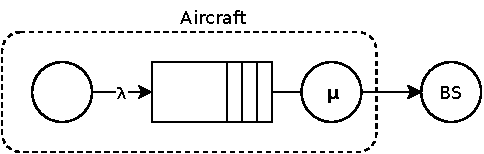
\includegraphics{img/model.pdf}
%   \caption{M/G/1 system for ACS}
%   \label{fig:model}
% \end{figure}

\section{Simulator}
\subsection{Software}
Simulator has been coded in C++ using the OMNeT++ environment and the INET framework. As data analysis tools we used a mixture of \textit{Python Pandas} and \textit{MS Excel}. 
\begin{figure}[H]
  \centering
  \begin{subfigure}[b]{0.45\textwidth}
    \centering
    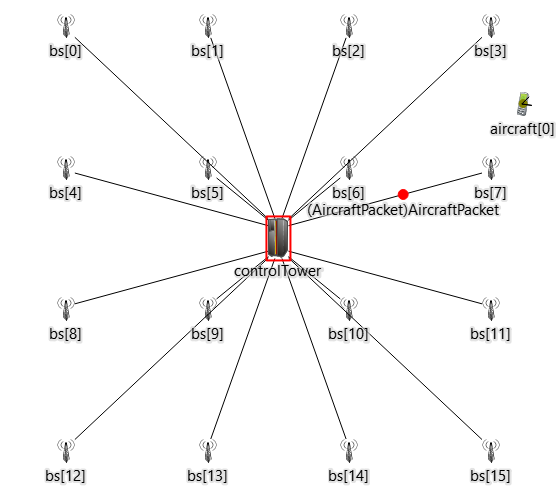
\includegraphics[scale=0.65]{img/Implementation.png}
    \caption{Communication Structure on Omnet++}
    \label{fig:aircraft-ned}
  \end{subfigure}
  ~
  \begin{subfigure}[b]{0.45\textwidth}
      \centering
      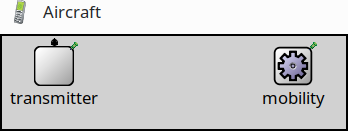
\includegraphics{img/aircraft-ned.png}
      \caption{Module structure of Aircraft}
      \label{fig:aircraft-ned}
  \end{subfigure}
\end{figure}
Transmitter implements the behaviour of AC described in \ref{Introduction}. Base Stations are only responsible for delivering packets to the control tower,
this communication is assumed to be instantaneous.
Regarding randomness, mobility module and the exponential interarrival time have their own stream of random numbers.
Moreover, repetitions are made independent by setting seeds of random generators equals to the repetition number. 

\subsection{Movement of AC}
Movement of AC is given by the following algorithm, implemented using the \texttt{TurtleMobility} module from INET:
\begin{itemize}
  \item generate a vector $\vec{s}$ such that $|\vec{s}| \in \mathcal{U}(0, M_{T}\sqrt{2})$ and $\angle{s} \in \mathcal{U}(0, 2\pi)$; upper bound of $\vec{s}$ is maximum possibile distance before AC surely wraps around;
  \item given that AC is in position $\vec{a}$, move to position $\vec{a} + \vec{s}$, at constant $v$ speed, possibly wrapping around at the edges of the simulated topology;
  \item once reached new position, re-do from the beginning;
\end{itemize}

This algorithm is equivalent to \texttt{Random WayPoint}, but takes in account the possibility of a wrap around.

\section{Verification}
\subsection{Code verification}
The simulator has been checked for bugs and memory leaks using Valgrind.

In order to verify the correctness of our code, we recorded the service time for a simulation and looked at a small time interval in order to spot abviously wrong situations.

\begin{figure}[H]
  \centering
  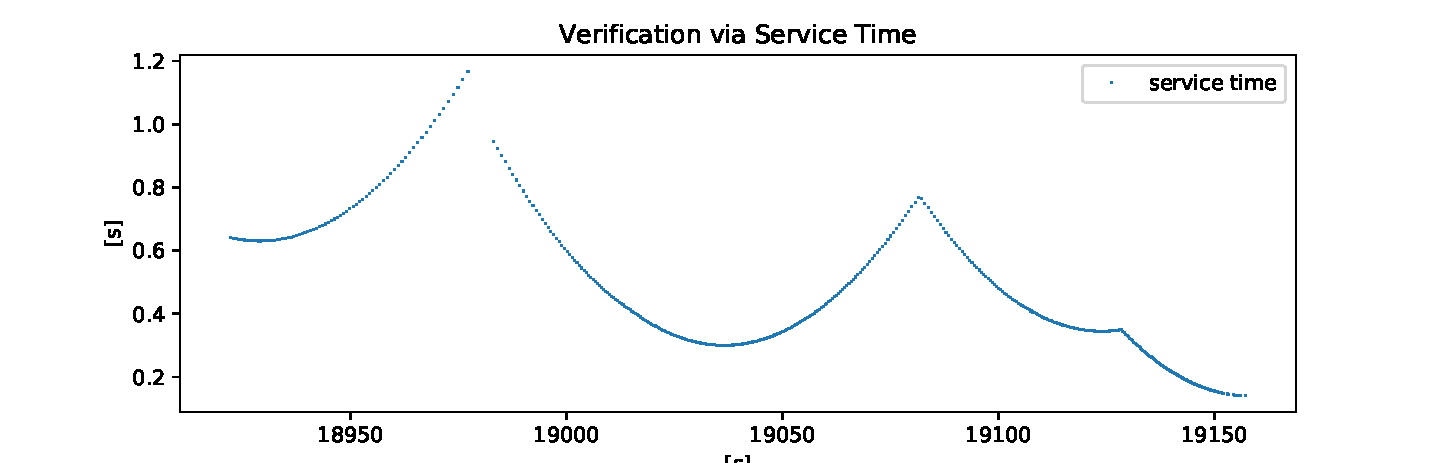
\includegraphics[scale=0.6]{img/verification-via-service-time.pdf}
  \caption{Service time during a test simulation}
  \label{fig:verification-via-service-time}
\end{figure}

We can see that:
\begin{itemize}
  \item service time has a paraboloid shape, which is expected since it is proportional with $d^2$, which $d$ increases linearly during time, because AC travel at costant speed;
  \item graph discontinuity, like the one between 18950 and 19000, represent the penalty time, which can be observed after an handover; service time correctly decreases after the handover;
  \item graph non derivability, like two points slightly before 19100 and 19150, represent the moment when AC randomly changes direction;
\end{itemize}

At this point, we are confident that the code for our simulator is correctly modeling the real world scenario, thus we can go through a more in-depth inspection by performing some validation test.

\subsection{Warm-Up study}
At the beginning of the simulation, the system could not be stable, and statistics recorded during this period of time produce meaningless results.
Thus, we measured the end to end delay of the system by stressing it with small interarrival time of $k=0.5$, running 20 independent simulations, and smoothing the value using a moving average with a window of 20k samples.
% k = 0.5, t = 16.95, p = 1 -- stress?

\begin{figure}[H]
  \centering
  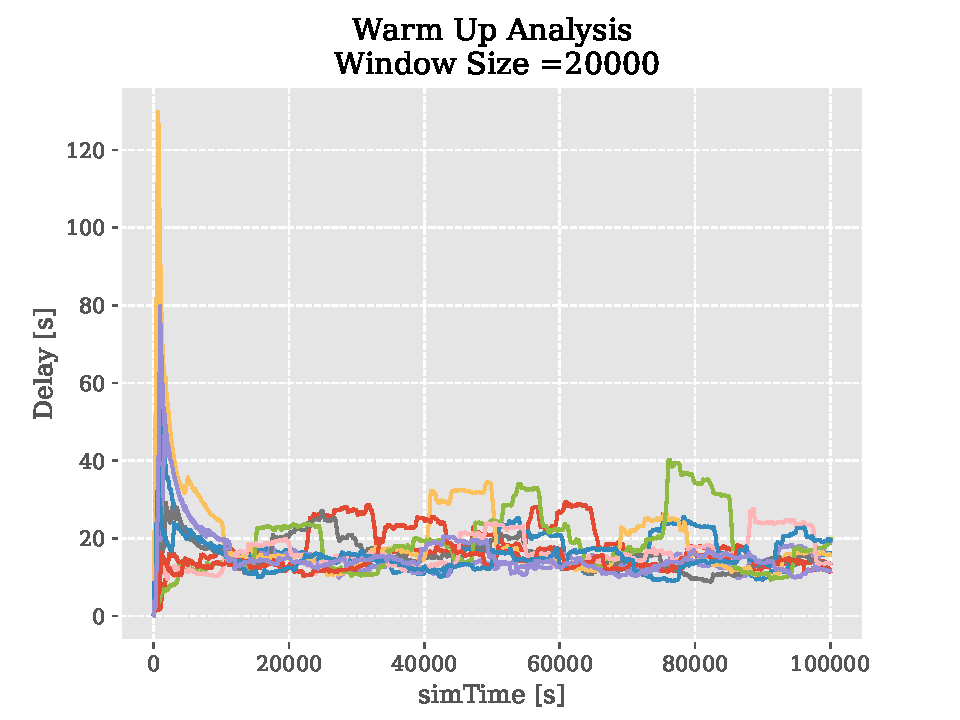
\includegraphics[scale=0.6]{img/warmup-study.pdf}
  \caption{Warmup study}
  \label{fig:warmup-study}
\end{figure}

From Figure~\ref{fig:warmup-study} we decided to use 10 ks as warmup time.

\section{Validation tests}
\subsection{Maximum distance considerations}
\label{sec:max-distance-considerations}
\begin{figure}[H]
  \centering
  \begin{subfigure}[b]{0.45\textwidth}
    \centering
    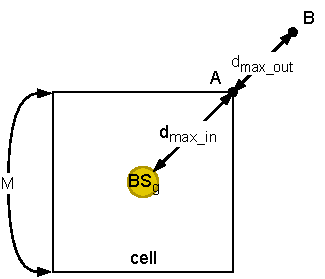
\includegraphics{img/dmax.pdf}
    \caption{Computation of $d_{max}$}
    \label{fig:dmax}
  \end{subfigure}
  ~
  \begin{subfigure}[b]{0.45\textwidth}
    \centering
    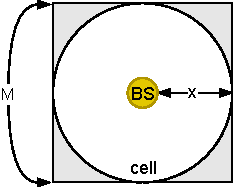
\includegraphics{img/d-simplified.pdf}
    \caption{Single-BS distance computation}
    \label{fig:d-simplified}
  \end{subfigure}
  \caption{Computation of distance between AC and BS}
  \label{fig:d}
\end{figure}

Service time depends on distance between AC and BS.
Distance between AC and BS, namely \emph{d}, belongs to interval $[ 0, d_{max} [$ where $d_{max}$ can be computed as $d_{max\_in} + d_{max\_out}$, where:
\begin{itemize}
  \item $d_{max\_in} = \frac{M \sqrt{2}}{2} $
  \item $d_{max\_out} = vt$
\end{itemize}

What is the worst case? Referring to Figure~\ref{fig:dmax}, let's assume that an AC is moving in direction $BS_g \rightarrow B$, and that, at a given time $t_g$, $\overrightarrow{AC} \in cell$ and $\overrightarrow{AC} - \overrightarrow{A} < \epsilon$ with $\epsilon$ small as you wish, eg. AC is at point A but still inside the cell where the nearest BS is $BS_g$; and let's assume that, at this time, AC initiates the handover procedure and discovers that the nearest BS is $BS_g$. Immediately after this handover procedure, performed without any penalty time, AC is out of the cell and will not initiate the handover procedure before $t$ time: this means that, when it is in point B, it has traveled for, $d_{max\_out} = v t$, since the last handover procedure, and that the longest distance $d_{max}$ between AC and BS is given by:

$$ d_{max} = \frac{M \sqrt{2}}{2} + vt $$

This result can be used to validate our simulator.

\subsection{Single-BS distance distribution computation}
\label{sec:singlebs-ddc}
In order to compute the distribution of service time, and to validate our model against a known queuing theory model, we had to make some simplifications for the computation of distance, and in particular: the cell around a single BS was used.

We want to compute $P\{D = x\}$, eg. probability that, picked a random position for AC inside the cell, distance $D$ between AC and BS equals to $x$.
As shown in Figure~\ref{fig:d-simplified}, intuition suggests that, with bigger circumferences (centered in BS) with radius $x$, in the real world, more points are suitable to satisfy $D = x$, thus $P\{D = x\}$ is proportional with circumference, which is proportional with radius.

However, for distances such that $d > \frac{M}{2}$, only arcs of that circumference which lay inside the square cell have to be taken in account in this computation.

So, a reasonable PDF for D is:

$$
f_D(x) = \begin{cases}
k \cdot 2 \pi x & \mbox{if } 0 \leq x \leq \frac{M}{2} \\
k \cdot \left( 2 \pi x - 8 x \cdot arccos \left(\frac{M}{2x}\right)\right) & \mbox{if } \frac{M}{2} \leq x \leq \frac{M \sqrt{2}}{2}\\
0 & otherwise
\end{cases}
$$

where
\begin{itemize}
  \item the first interval represents the probability of AC laying over a circumpherence fully inside the square cell (eg. blue);
  \item the second interval represents the probabilty of AC laying over the arcs given by the intersection of a circumpherence partially outside the square cell, and the square cell itself (eg. red);
  \item $k$ has been computed using the normalization condition and is equal to $k = 1.6 \times 10^{-9}$;
\end{itemize}

Once we know the distribution for distance D, we can compute the distribution for service time S:
% thanks to both Pietro and WolframAlpha
% only two can be 100% sure of this computation, and I still have some doubts about the second
$$
f_S(s) = \begin{cases}
\frac{\pi}{TM^2}  & \mbox{if } 0 \leq s \leq \frac{TM^2}{4} \\
\frac{\pi}{TM^2} - \frac{4}{TM^2} arccos\left( \frac{M}{2} \sqrt{\frac{T}{s}} \right) & \mbox{if } \frac{TM^2}{4} \leq s \leq \frac{TM^2}{2} \\
0 & otherwise
\end{cases}
$$

\begin{figure}[H]
  \centering
  \begin{subfigure}[b]{0.45\textwidth}
    \centering
    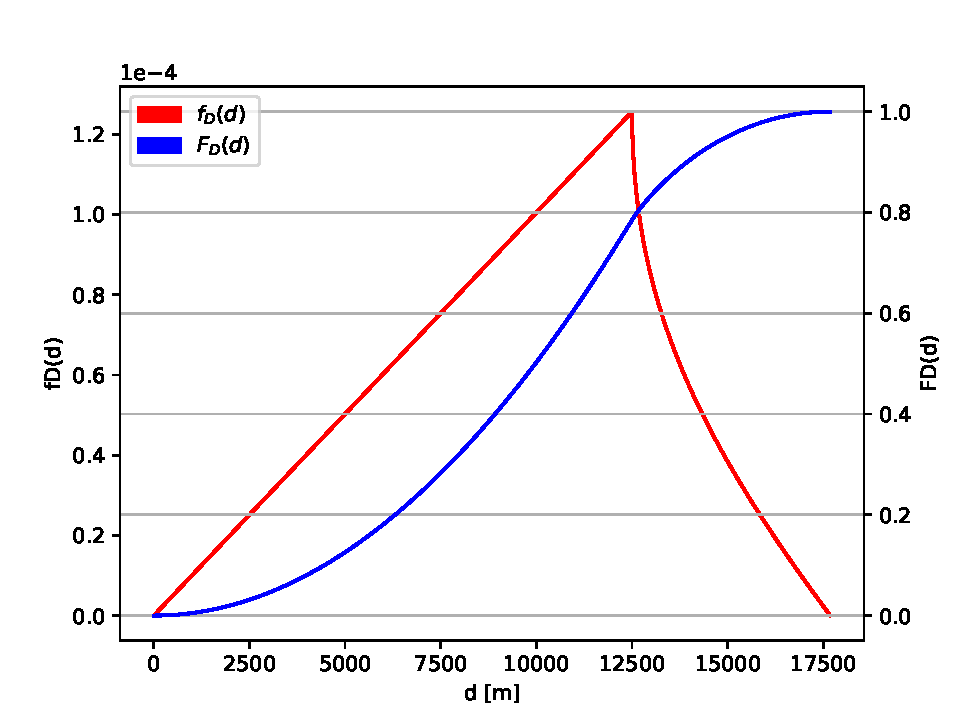
\includegraphics[width=\textwidth]{img/distance.pdf}
    \caption{Theoretical PDF and CDF of distance}
    \label{fig:pdfcdf-distance}
  \end{subfigure}
  ~
  \begin{subfigure}[b]{0.45\textwidth}
    \centering
    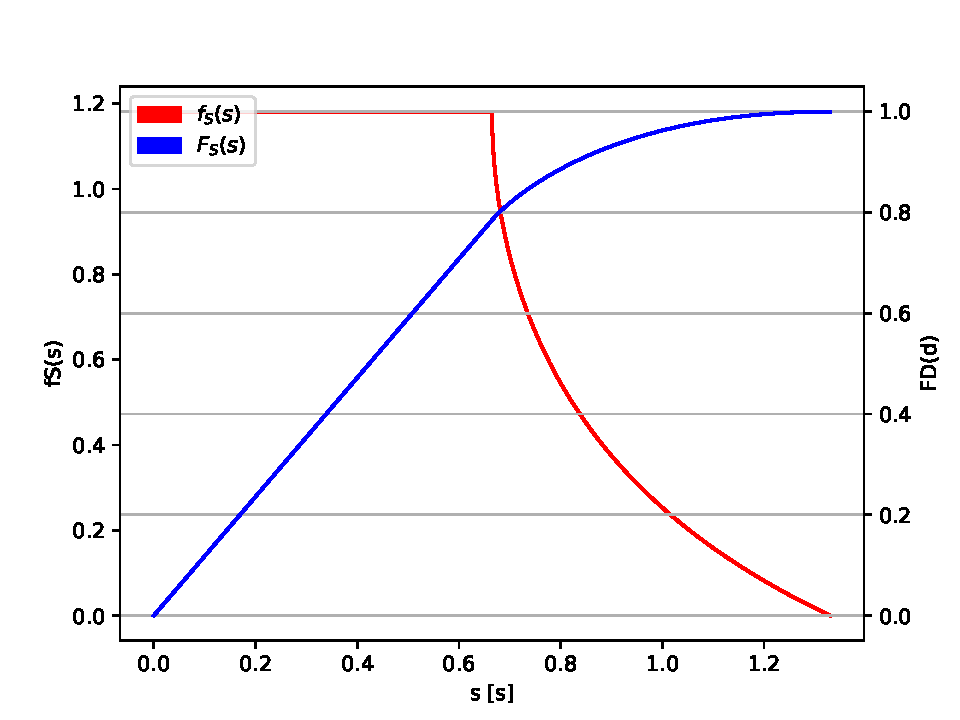
\includegraphics[width=\textwidth]{img/servicetime.pdf}
    \caption{Theoretical PDF and CDF of service time}
    \label{fig:pdfcdf-servicetime}
  \end{subfigure}
  \caption{Theoretical distribution of distance and service time}
  \label{fig:d}
\end{figure}

This result can be used to validate our simulator.

\section{Validation experiments}
\subsection{Maximum distance considerations}
Using results from Section~\ref{sec:max-distance-considerations}, we ran 10 independent simulations, with 5 different handover periods $t$, and sampled maximum distance.
Then we compared the samples with our theoretical computations, and, as we can see from Figure~\ref{fig:dmax-validation}, the experiment always confirmed the validity of our simulator.
% for all the measurements, see DistanceValidation.xlsx
\begin{figure}[H]
  \centering
  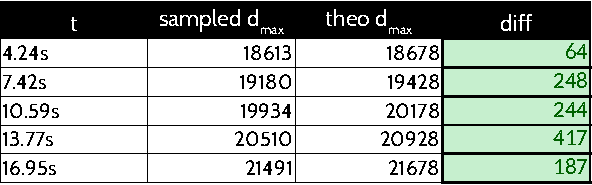
\includegraphics[scale=0.8]{img/dmax-validation.pdf}
  \caption{Maximum distance sampled between an AC and the connected BS [m]}
  \label{fig:dmax-validation}
\end{figure}

\subsection{Single-BS distance distribution computation}
\subsubsection{M/D/1}
We ran 30 independent simulations, keeping the AC at a fixed distance from a BS, and sampled the performance indexes.
Then, we compared them with those computed using Pollaczek and Khinchin’s formula.

\subsubsection{M/G/1}
We ran 30 independent simulations, and sampled distance and the performance indexes.

Using results from Section~\ref{sec:singlebs-ddc}, we compared the samples of distance and service time with our theoretical distributions using QQ plots.

\begin{figure}[H]
  \centering
  \begin{subfigure}[b]{0.45\textwidth}
    \centering
    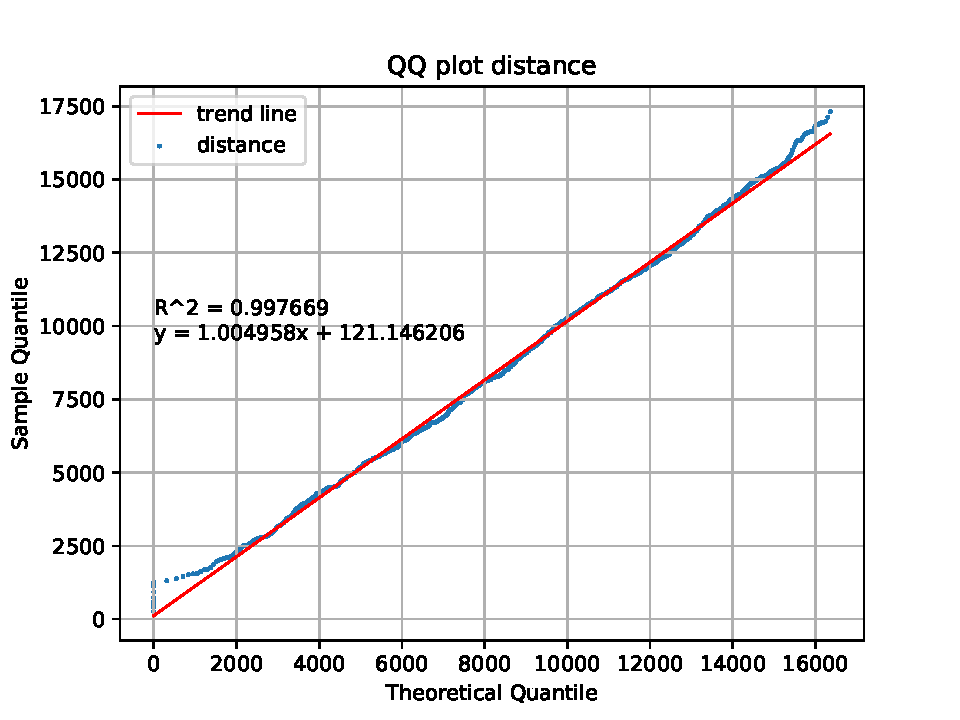
\includegraphics[width=\textwidth]{img/qq-distance.pdf}
    %\caption{Theoretical PDF and CDF of distance}
    \label{fig:qq-distance}
  \end{subfigure}
  ~
  \begin{subfigure}[b]{0.45\textwidth}
    \centering
    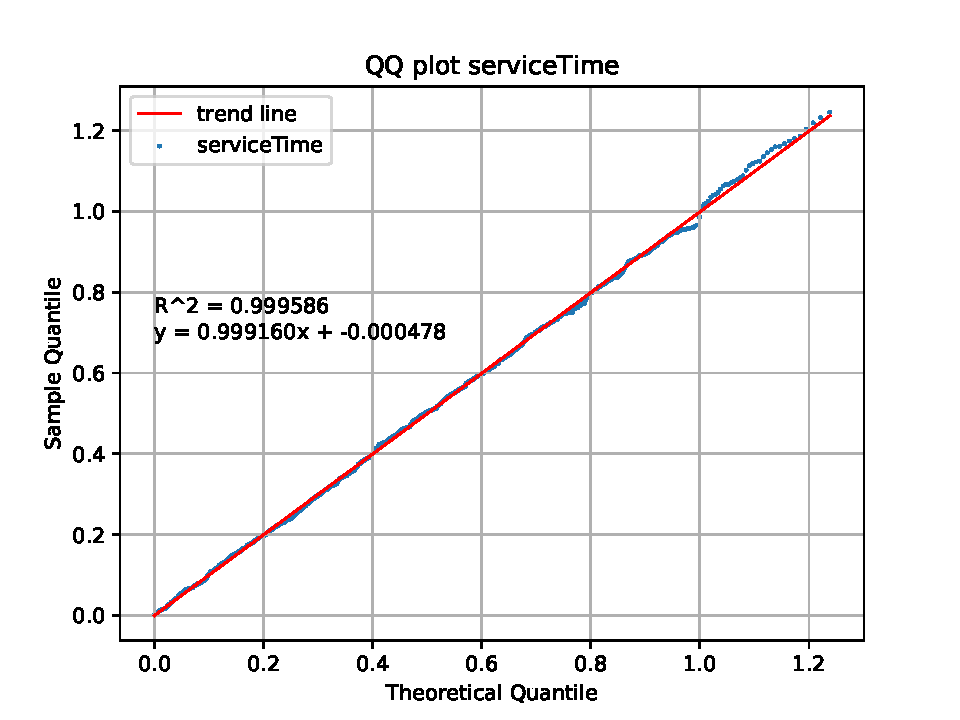
\includegraphics[width=\textwidth]{img/qq-servicetime.pdf}
    %\caption{Theoretical PDF and CDF of service time}
    \label{fig:qq-servicetime}
  \end{subfigure}
  \caption{QQ plots for fitting distance and service time distribution}
  \label{fig:d}
  \label{fig:qqplots}
\end{figure}

Once asserted the validity of the distribution, as can be seen in Figure~\ref{fig:qqplots}, we compared the measured performance indexes with those computed using PK's formula.

\begin{figure}[H]
  \centering
  \begin{subfigure}[b]{0.40\textwidth}
    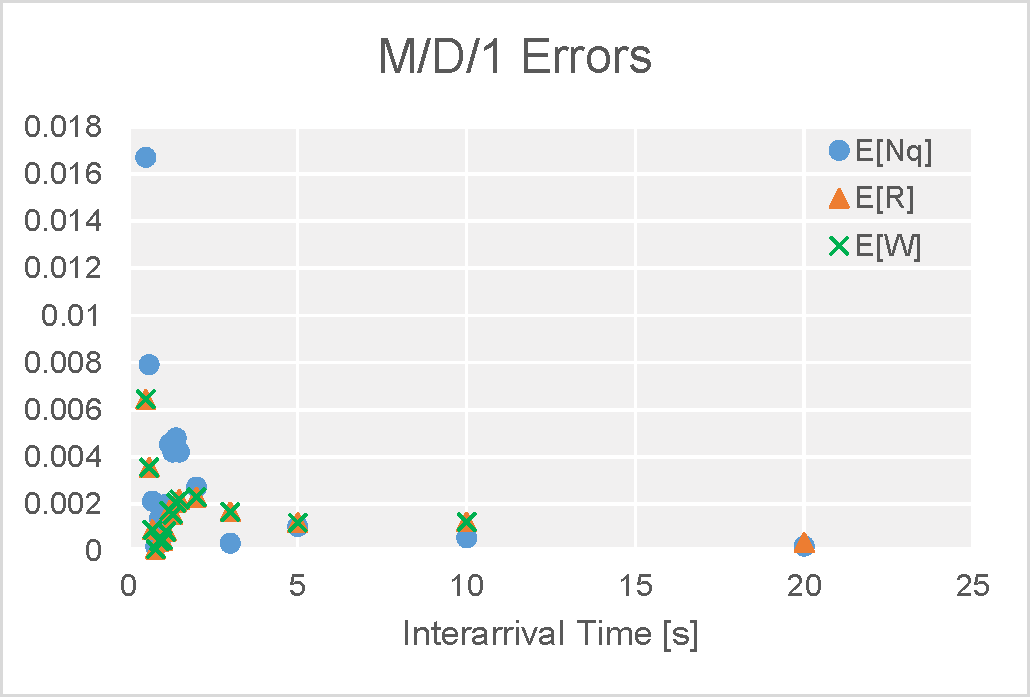
\includegraphics[width=\textwidth]{img/MD1.pdf}
    \caption{M/D/1}
  \end{subfigure}
  ~
  \begin{subfigure}[b]{0.40\textwidth}
    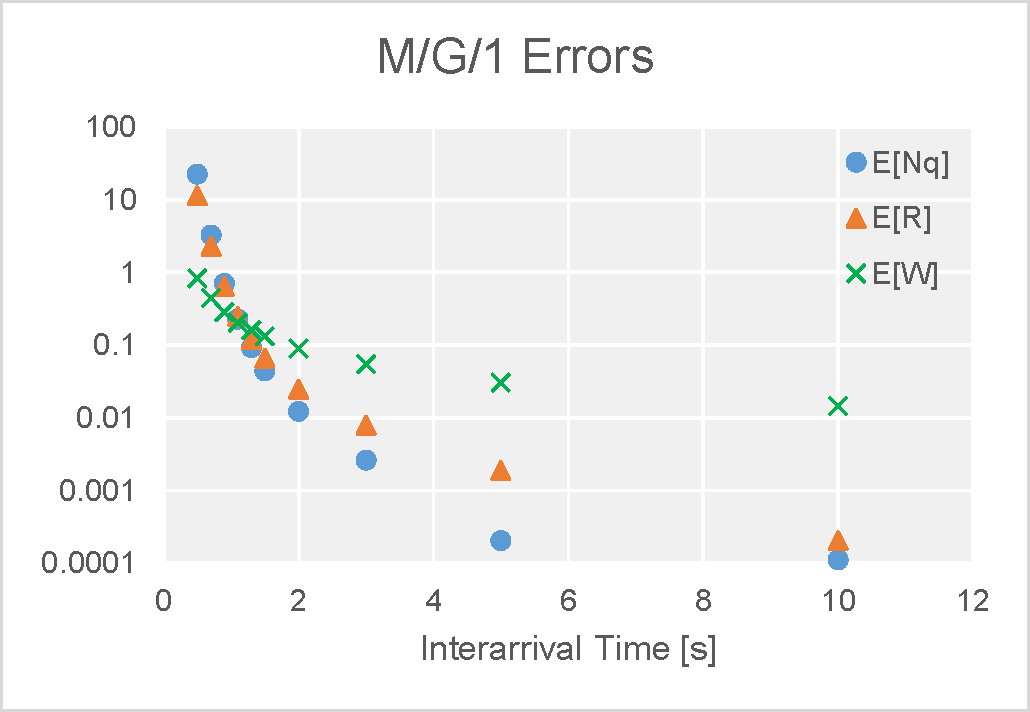
\includegraphics[width=\textwidth]{img/MG1.pdf}
    \caption{M/G/1}
  \end{subfigure}
  \caption{Measured and theoretical performance indexes error}
  \label{fig:perf-index-error}
\end{figure}

As we can see in Figure~\ref{fig:perf-index-error}, errors are small compared to the expected values, except for those closer to smaller interarrival time $k$, when the system tends to be less stable.

As we can see, this experiment confirmed the validity of our simulator.

\subsection{Handover convenience}
\label{sec:handover-convenience}
Last test was on the handover convenience: it is straightforward that we want

$$ s[t] \geq s[t + 1] $$

for each $t, t + 1$ such that and handover has been performed in between, eg. service time never increases after an handover. We ran 10 independent simulations which always complied with the expected results.
This experiment confirmed the validity of our simulator.

\section{Experiments}
Once validated the simulator, experiments were carried out, in order to study the system performances, for what concerns the end-to-end delay of packets delivery, and the queues length.

For every parameter, we run 30 independent simulations.

\begin{figure}[H]
  \centering
  \begin{tabular}{| c | c | c | c |}\hline
    \multicolumn{2}{|c|}{parameter} & values & unit \\ \hline
    interarrival time & \texttt{k} & \texttt{\{ 0.5, 0.75, 1, 1.25, 1.5, 1.75, 2 \}} & s \\ \hline
    handover period & \texttt{t} & \texttt{\{ 4.24, 7.42, 10.59, 13.77, 16.95 \}} & s \\ \hline
  \end{tabular}
\end{figure}

More in detail:
\begin{itemize}
  \item we would like to have an AC produce its position at most every 2 s, for air traffic control necessities.
  We analyzed $k$ values with a lower bound of 0.5 because, at that edge, it started to become unstable due to very high utilization $\rho$;
  \item we would like to check for an handover neither when the AC is too close to a cell edge, nor when it is too far.
  Fixing these values at a reasonable distance of 1km and 4km, and dividing the interval in 5 chunks, we found the values for $t$;
\end{itemize}

\subsection{First experiments}
As we can see from graphs in Figure~\ref{fig:result-0}, the fact that interarrival time has a costant or exponential distribution only slightly changes the system behavior, at such a point that it can be ignored.

Anyhow we see that both end-to-end delay and queue length highly depend on the mean interarrival time: lower mean interarrival times lead to higher delays and longer queues, while higher mean interarrival times lead to lower delays and shorter queues.
This fact can be physically explained with service center usage: the lower the interarrival time, the higher is the system usage, and with $k \approx 0.5s$, $\rho \approx 0.9$.

Using a long handover check period allows the AC to travel further from the BS it is connected to in that moment, thus giving an higher service time, but we already put an upper bound to this value by chosing $t = 16.95s$, which corresponds to a worst case of approximately $20 km$.
What we expected is that, with smaller handover check periods, we could improve our system's performances by finding a proper tradeoff, but graphs show that the best system performances are obtained with higher

This means that the penalty time, which has a fixed value, is particularly relevant in our analysis, and is of minor influence, and almost trascurable in certain cases, only as long as $t$ is an order of magnitude bigger than $p$.

\begin{figure}[H]
  \centering
  \begin{subfigure}[b]{.45\textwidth}
    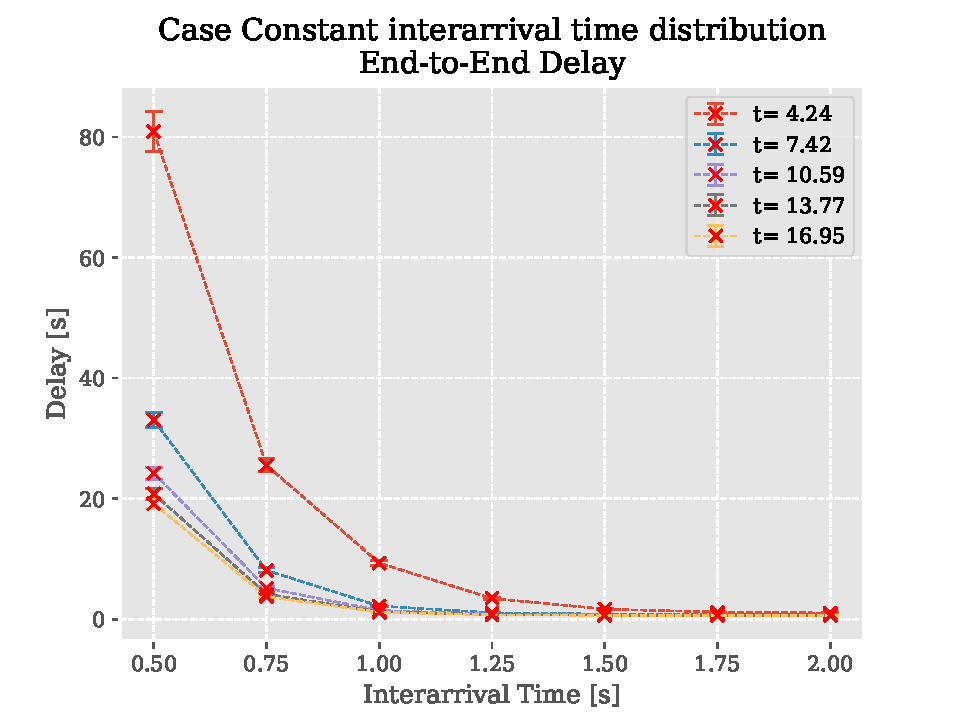
\includegraphics[width=\textwidth]{img/DelayP2Const.pdf}
    %\caption{}
    \label{fig:exp:const:delay}
  \end{subfigure}
  ~
  \begin{subfigure}[b]{.45\textwidth}
    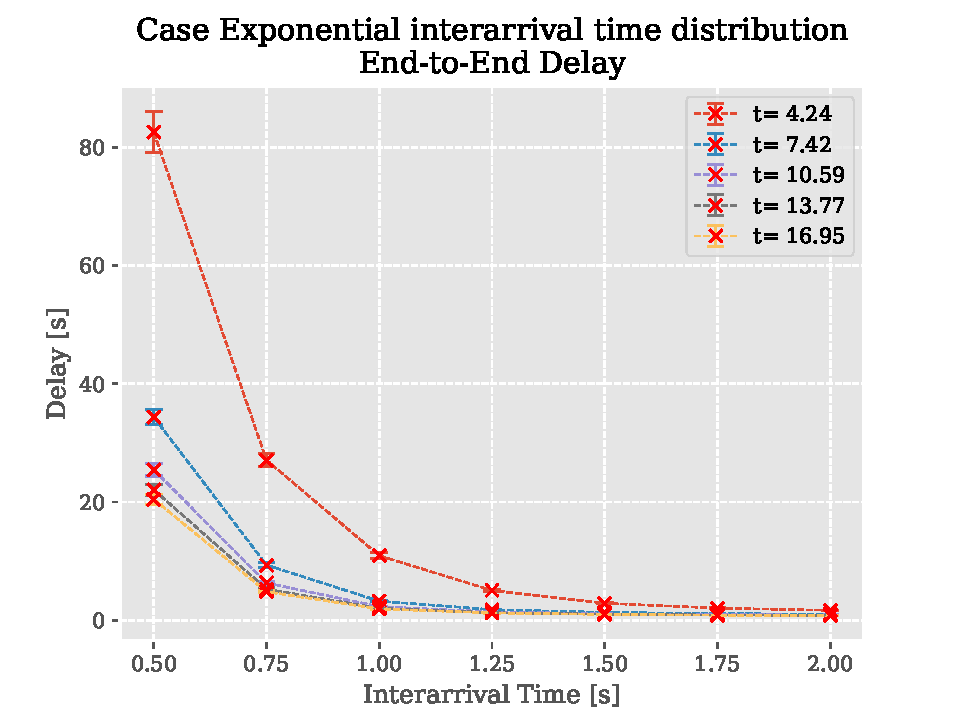
\includegraphics[width=\textwidth]{img/DelayP2Exp.pdf}
    %\caption{}
    \label{fig:exp:exp:delay}
  \end{subfigure}
  \\
  \begin{subfigure}[b]{.45\textwidth}
    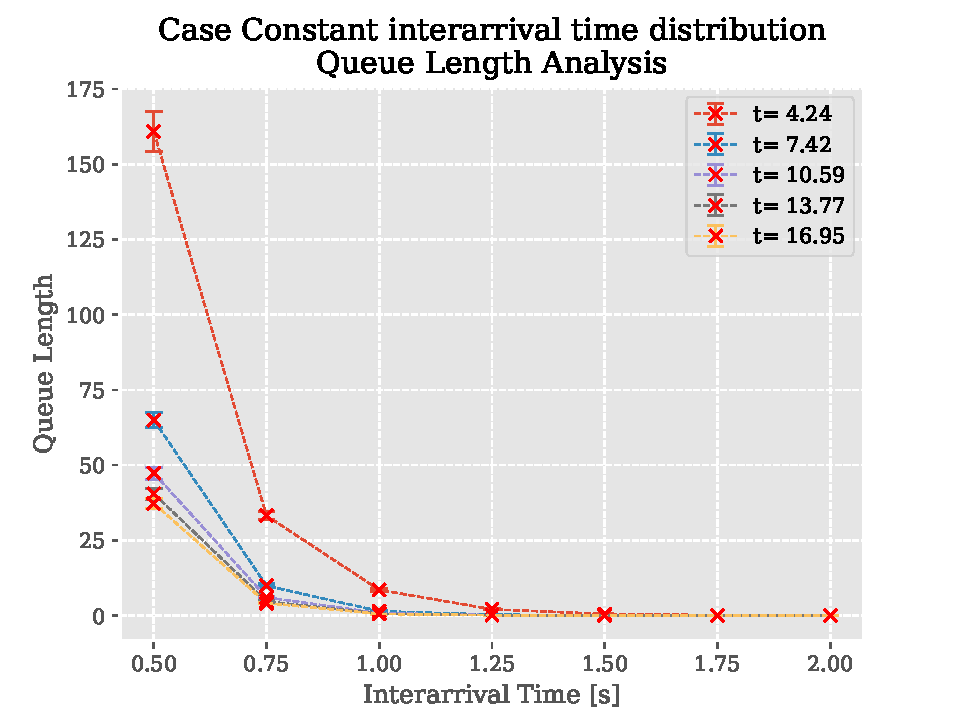
\includegraphics[width=\textwidth]{img/QueueLengthP2Const.pdf}
    %\caption{}
    \label{fig:exp:const:queue}
  \end{subfigure}
  ~
  \begin{subfigure}[b]{.45\textwidth}
    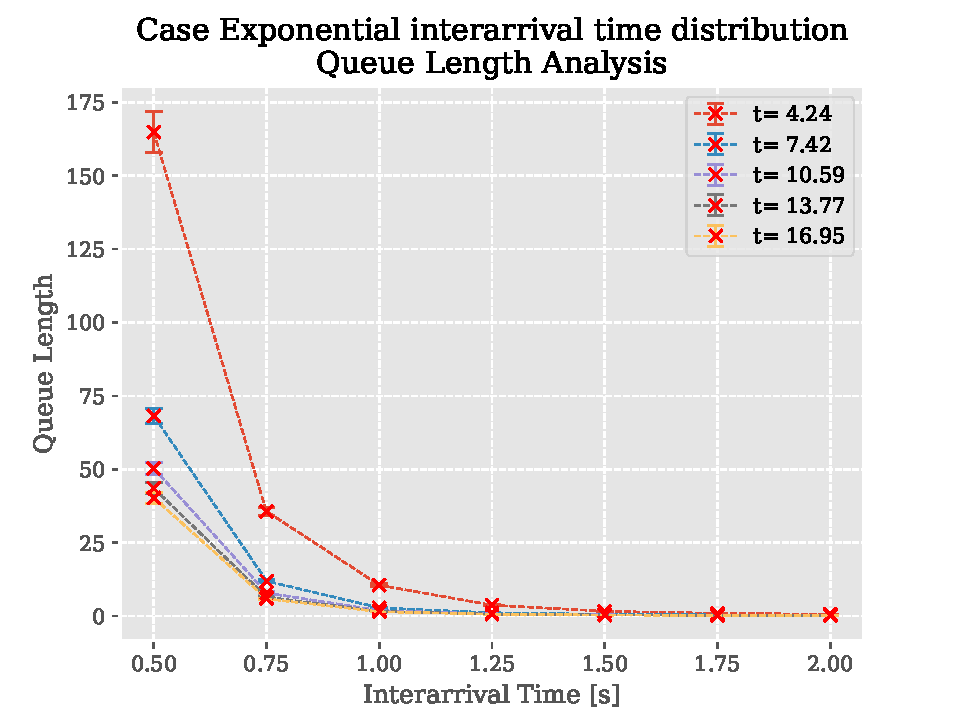
\includegraphics[width=\textwidth]{img/QueueLengthP2Exp.pdf}
    %\caption{}
    \label{fig:exp:exp:queue}
  \end{subfigure}
  \caption{Results: on the left, costant interarrival time; on the right, exponential interarrival time.}
  \label{fig:result-0}
\end{figure}

\subsection{Further analysis}
Since end to end delay graph and queue length graph have a similar shape, we thought that higher end to end delay mainly depended on waiting time (eg. time that a packet has to wait in the queue before being served), so we decided to further investigate and compare the amount of response time with the amount of waiting time.
Figure~\ref{fig:result-1}, bars of response time in red and waiting time in various colors are overlapped, and we can clearly see that packets spend most of their response time in the queue. 

So we can assert that the proper way to improve this system's performances is by lowering the waiting time over response time ratio.

\begin{figure}[H]
  \centering
  \begin{subfigure}[b]{.45\textwidth}
    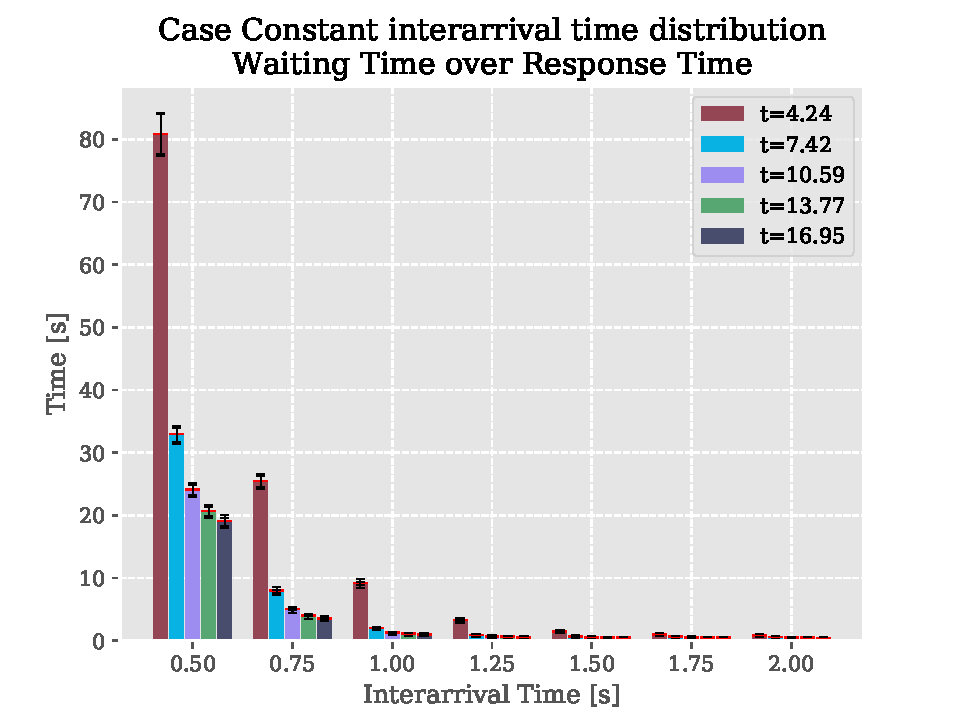
\includegraphics[width=\textwidth]{img/WaitingTimeOverResponseTimeP2Const.pdf}
    %\caption{}
    \label{fig:exp:const:wor}
  \end{subfigure}
  ~
  \begin{subfigure}[b]{.45\textwidth}
    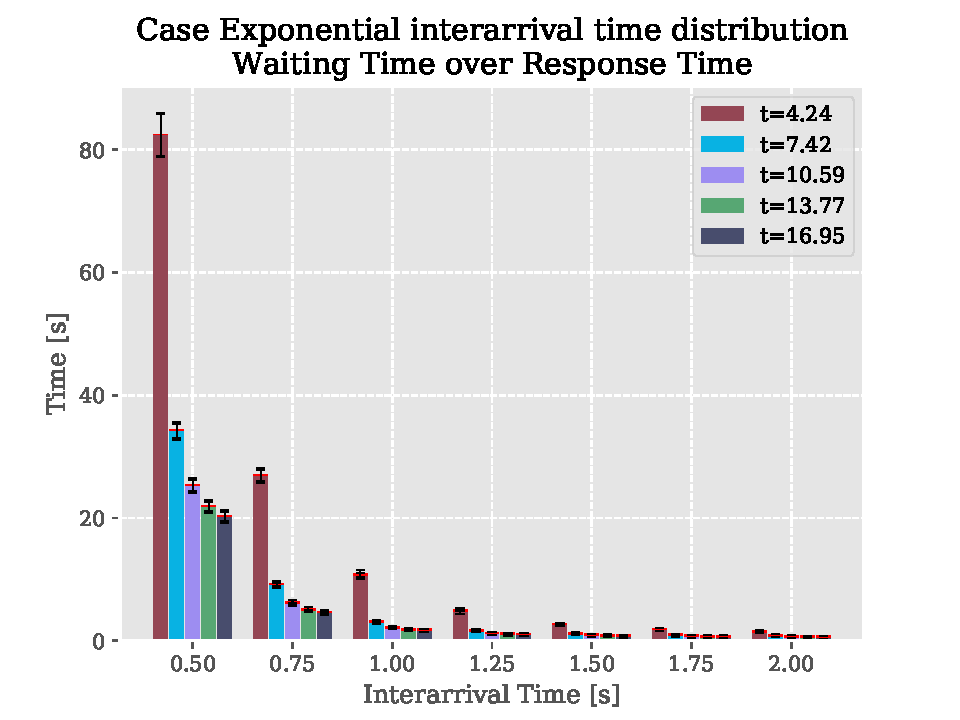
\includegraphics[width=\textwidth]{img/WaitingTimeOverResponseTimeP2Exp.pdf}
    %\caption{}
    \label{fig:exp:exp:wor}
  \end{subfigure}
  \caption{Fraction of waiting time over response time}
  \label{fig:result-1}
\end{figure}

\subsection{Possible improvements}
In order to make a quick test and confirm the validity of this intuition, we assumed, for a moment, that $p$ could be lowered from $2s$ to $1s$.
As can be seen in Figure~\ref{fig:result-2}, behavior has a similar shape, but different magnitude, and this confirmed the intuition.
Note that, since exponential and costant interarrival time show almost the same behavior, we investigated only the former.

\begin{figure}[H]
  \centering
  \begin{subfigure}[b]{.3\textwidth}
    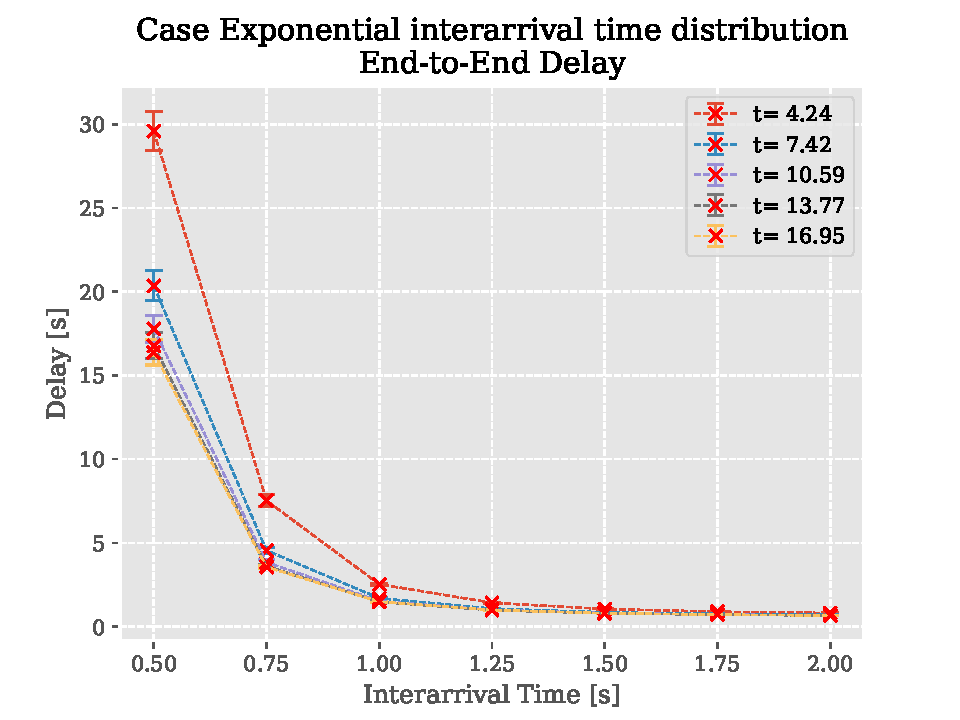
\includegraphics[width=\textwidth]{img/DelayP1Exp.pdf}
  \end{subfigure}
  ~
  \begin{subfigure}[b]{.3\textwidth}
    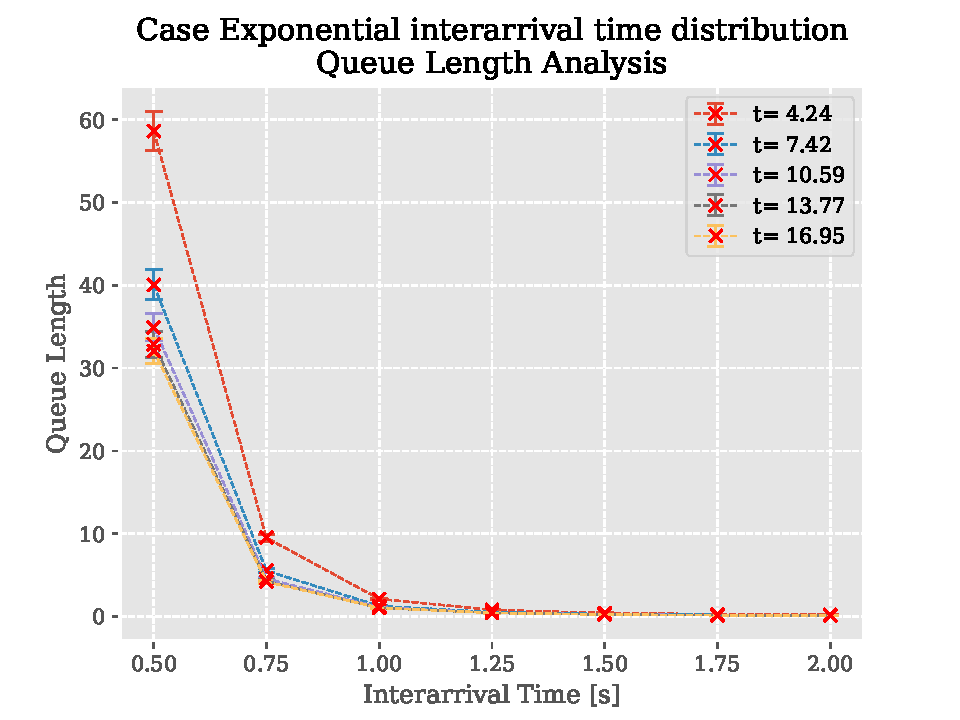
\includegraphics[width=\textwidth]{img/QueueLengthP1Exp.pdf}
  \end{subfigure}
  ~
  \begin{subfigure}[b]{.3\textwidth}
    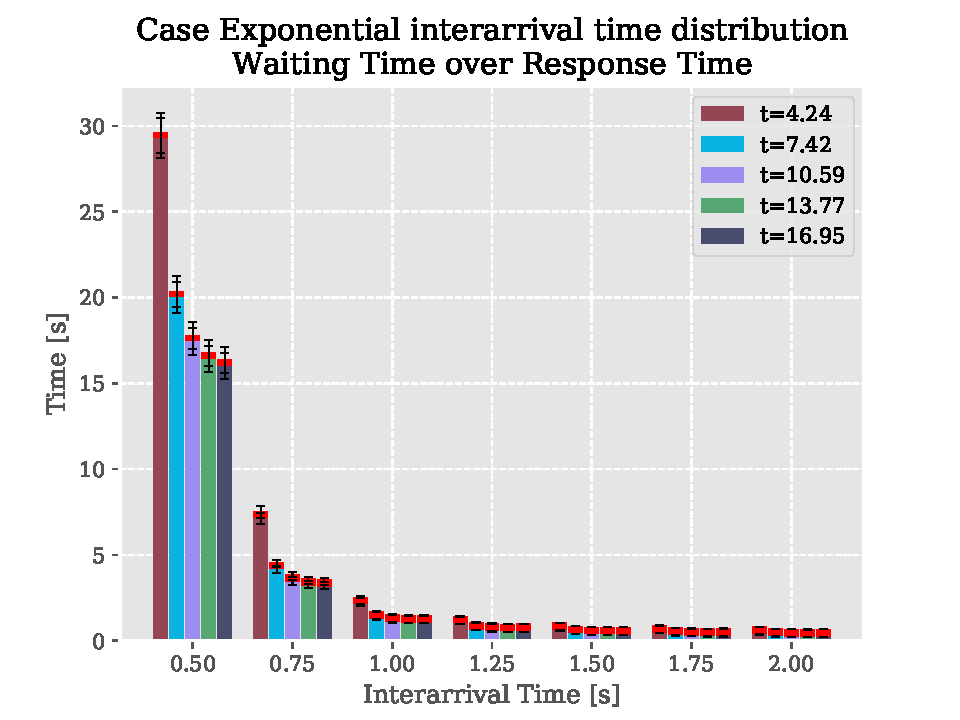
\includegraphics[width=\textwidth]{img/WaitingTimeOverResponseTimeP1Exp.pdf}
  \end{subfigure}
  \caption{Experiments performed with a reduced waiting time}
  \label{fig:result-2}
\end{figure}

\section{Factorial Analysis}
Results clearly show that interarrival time has a huge impact on our system, so we expect that performing a factorial analysis should yield the same result. 
\subsection{Method}
Our study was conducted for both constant and exponential case on the 2 requested factors, interarrival time \textbf{k} and handover period \textbf{t}, adding penalty time \textbf{p} as third factor,
using 30 replicas.  

Summing up, we have $2^3*30 = 240$ configurations per case, exploring the combinations of the following factors' extremes:

\begin{figure}[H]
  \centering
  \begin{tabular}{| c | c | c | c |}\hline
    \multicolumn{2}{|c|}{parameter} & values & unit \\ \hline
    interarrival time & \texttt{k} & \texttt{\{ 0.5, 2 \}} & s \\ \hline
    penality time & \texttt{p} & \texttt{\{ 1, 2 \}} & s \\ \hline
    handover period & \texttt{t} & \texttt{\{ 4.24, 16.95 \}} & s \\ \hline
  \end{tabular}
\end{figure}

During analysis we realize that the assumptions that residuals are IID normal RVs with null mean and costant standard deviation do not hold. 
In detail, comparing residuals quantiles and normal quantiles leads to a qq plot with poor linear behaviour ( $R^2 = 0.6704$ ). To fix this issue, we tested 
different transformations and the best result is achieved using the following:

$$y' = log(y)$$

Thus, residuals become normal IID RVs with constant standard deviation since plots of Residuals vs Average Predicted Value and Residuals Vs Experiment Number do not show any particular trend.

\subsection{Results}
Once hypothesis are met, we are sure that nonlinear regression model works and leads to the result showed in \ref{fig:faexp} and \ref{fig:faconst}

\begin{figure}[H]
  \centering
  \begin{subfigure}[b]{.45\textwidth}
    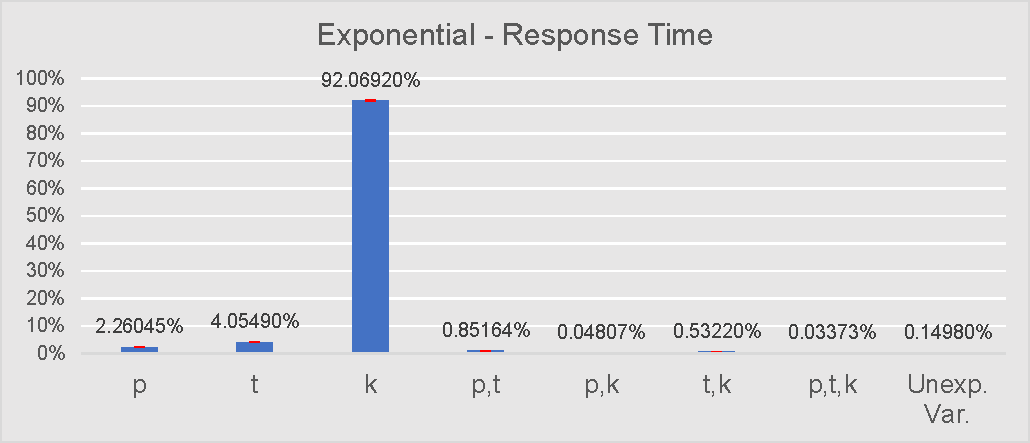
\includegraphics[width=\textwidth]{img/FactorAnalysisResponseTimeEXP.pdf}
  \end{subfigure}
  ~
  \begin{subfigure}[b]{.45\textwidth}
    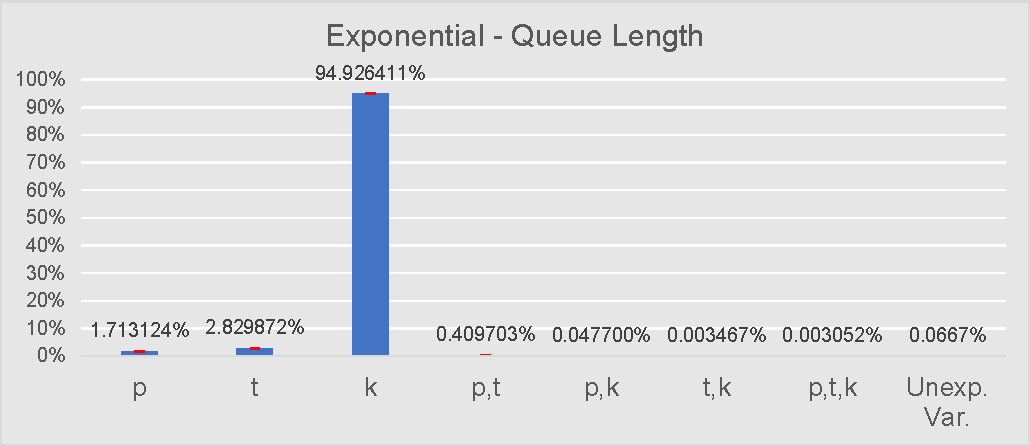
\includegraphics[width=\textwidth]{img/FactorAnalysisQueueLengthEXP.pdf}
  \end{subfigure}
  \caption{Factorial analysis on response time and queue length of case exponential }
  \label{fig:faexp}
\end{figure}

\begin{figure}[H]
  \centering
  \begin{subfigure}[b]{.45\textwidth}
    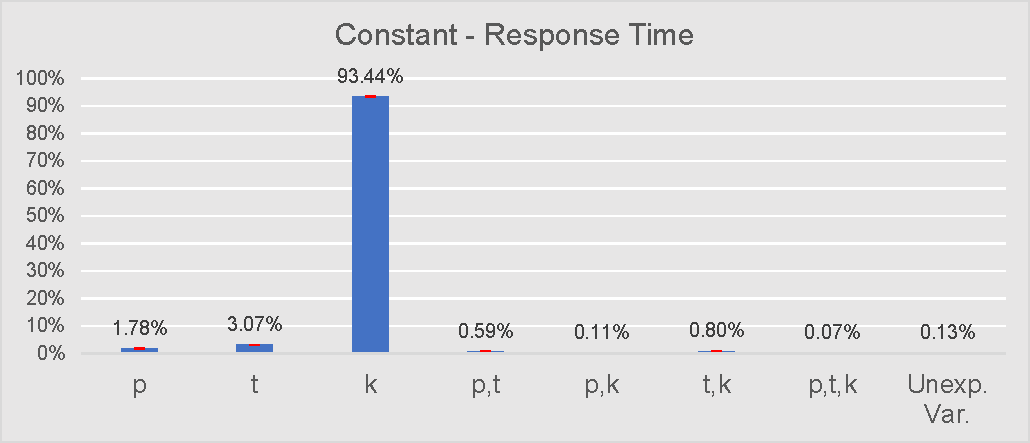
\includegraphics[width=\textwidth]{img/FactorAnalysisResponseTimeCONST.pdf}
  \end{subfigure}
  ~
  \begin{subfigure}[b]{.45\textwidth}
    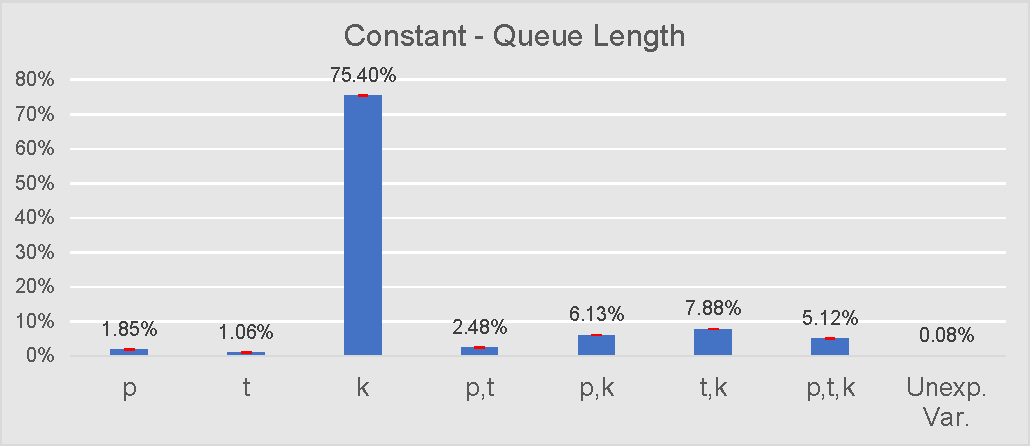
\includegraphics[width=\textwidth]{img/FactorAnalysisQueueLengthCONST.pdf}
  \end{subfigure}
  \caption{Factorial analysis on response time and queue length of case constant }
  \label{fig:faconst}
\end{figure}

It is pretty clear that varying the interarrival time leads to huge changes in both response time and queue length, while other factors are not so relevant as the first one.
Interplays are almost not present, except for the queue length of the constant interarrival time distribution case. The latter could be attributed to the fact that some factors' combinations
leads to $E[N_q] = 0$, i.e. :

\begin{figure}[H]
  \centering
  \begin{tabular}{| c | c | c | c |}\hline
    p & t & k & unit\\ \hline
    1 & 4.24 & 2 & s \\ \hline
    1 & 16.95 & 2 & s \\ \hline
    2 & 16.95 & 2 & s \\ \hline
  \end{tabular}
\end{figure}

For example, if we change $ t = 4.24s , k = 0.5s $ to $ t = 16.95s , k = 2s $, then $E[N_q]$ goes from $ \sim 55 $ to $0$ for $ p = 1s $ and from $\sim 160 $ to $0$ for $ p = 2 $, then $7.8815\%$ of t,k interplay is justified. 
This behaviour does not appear in other cases because mean values of those same combinations are still low but not completely null. 
\section{Conclusions}

\end{document}
